
\chapter{Results}


XXX - CV needs pictures. 
look at 5.5 pixels and say why that bad, visualize maybe
single image for match not side by side. - not clear what its finding, but it is robust which is nice - try ask what are these dots... what are keypoints 
- GitHub link for code. Mentionthis is how it was implemented, not flow diagram. So when someone goes on Github they know whats going on.
Crop Earth 
overlap relative to my baseline image 972. no 1080.  CTRL F 1080.
xxx - show matches black and white. / xxx show image overlay.

\section{Key Metric Analysis}

This section presents the results achieved by the navigation system under optimal conditions across various challenging datasets. The analysis focuses on the system's performance in terms of accuracy, efficiency, and generalizability, providing insights into its applicability in real-world UAV navigation scenarios. More information about the testing setup is provided in \ref{chap:Testing}

\subsection{Key Performance Metrics}

The system's performance across the five diverse datasets—CITY1, CITY2, ROCKY, DESERT, and AMAZON—is evaluated based on Accuracy and Runtime.

\textbf{Accuracy} is assessed in two primary ways:

1. \textit{Absolute Radial Error (RMSE)}: Measured in the estimates radial metres from the ground truth, averaged for the dataset. This metric provides a tangible understanding of the error magnitude and the system's responsiveness to movement size. Additionally, it may be represented per-image, in pixels or in axial components, offering an intuition of error size relative to the fixed resolution of 1920x972 pixels.

2. \textit{Relative Radial Error}: Expressed as the per image Absolute Radial Error as a percentage of the ground truth radial change in distance, averaged for the dataset. The ground truth radial change is the magnitude of the translation vector from the reference image's center to the current image's center, both measured in meters. This normalized metric allows for a clearer understanding of the system's accuracy relative to the movement size. It may also be represented per-image or in axial components.


\textbf{Runtime} is evaluated in three stages:
1. \textit{Mean Add Time (With GNSS)}: The average time required to add one image to the pipeline, including streaming the image and extracting its features. This time determines the system's processing rate while GNSS signals are available after parameter inference has concluded.

2. \textit{Mean Parameter Inference Time (With GNSS)}: The average time needed to infer the pixel-to-meter conversion factor per image. This includes processing the entire pipeline (finding the best match and subsequent transformation estimation) to estimate the UAV's position, and computing linear regression by leveraging the ground truth once at the end of the mode. Adding this to the add time provides the total time to process an image when GNSS is available and parameter inference is active. Inference mode is active for the first five images, since further tests continued to limit the reference image capture rate while producing negligible improvements in accuracy.

3. \textit{Mean Location Inference Time (Without GNSS)}: The average time taken to infer the UAV's location when GNSS signals are lost. Measured per image, this time encompasses processing the entire pipeline to estimate the UAV's position. This metric is critical as it determines how quickly a pilot can correct any path deviations to prevent further drift.


The results show that the system achieves consistent accuracy and runtime performance across each dataset. This section details the performance metrics for each dataset, while the following sections analyze the sources of error where applicable.

In terms of accuracy, all datasets achieved a mean radial error below 1\% of the ground truth distance, a mean pixel error being below 1.05 pixels a mean meter error below 3.2 meters. As the percentage error of the ground truth distance is the most fair metric, the order of average performance is therewith evaluated. The CITY2 dataset showed the best performance, followed by the DESERT dataset, then the AMAZON dataset, then the CITY1 dataset, and finally, with a large difference in performance, the ROCKY dataset. 

In terms of maximum single image errors across datasets, the maximum error ocurred in the ROCKY dataset. This maximum radial error 6.21\% of the ground truth distance, which corresponds to 27.54 meters or 4.93 pixels. In terms of maximum percentage error, the CITY2 dataset showed the best performance, followed by the DESERT dataset, then the CITY1 dataset, then the AMAZON datast, and finally, with a large difference in performance, the ROCKY dataset.


In terms of mean runtimes, the mean add time across datasets was below 0.6 seconds, the mean parameter inference time was below 1.4 seconds, and the mean location inference time was below 1.3 seconds. This indicates that the system is on average able to maintain real-time performance while inference mode is on, with the sum of the parameter inference and add times being below 2 seconds. Further, the the location inference time is below 2 seconds.

However, when looking at maximum runtime, the system produced runtimes over 2 seconds while inference mode was on. While off, the system maintained real-time performance. This means that real-time performance was not met while inference mode was on. However, inference mode is only applied to the first few images, meaning the time may be caught up relatively quickly while inference mode is off, as images will be stored prior to their usage in the pipeline. This basically means if the system is behind at some point, the images are still there for later catchup. 




% Table: Mean Radial Errors
\begin{table}[H]
    \centering
    \caption{\textbf{Mean Radial Errors}}
    \label{tab:mean_radial_errors}
    \begin{tabular}{|l|c|c|c|c|c|}
    \hline
    & \textbf{CITY1} & \textbf{CITY2} & \textbf{ROCKY} & \textbf{DESERT} & \textbf{AMAZON} \\
    \hline
    \makecell{\textbf{Percentage Radial Error (\%)}} & 0.4001 & 0.2290 & 1.9154 & 0.2515 & 0.3811 \\
    \hline
    \makecell{\textbf{Pixel Error}} & 0.8196 & 0.6114 & 1.0520 & 0.5668 & 0.3919 \\
    \hline
    \makecell{\textbf{Meter Error}} & 4.7978 & 2.7576 & 5.8822 & 2.3573 & 2.5336 \\
    \hline
    \end{tabular}
\end{table}

% Table: Maximum Radial Errors
\begin{table}[H]
    \centering
    \caption{\textbf{Maximum Radial Errors}}
    \label{tab:max_radial_errors}
    \begin{tabular}{|l|c|c|c|c|c|}
    \hline
    & \textbf{CITY1} & \textbf{CITY2} & \textbf{ROCKY} & \textbf{DESERT} & \textbf{AMAZON} \\
    \hline
    \makecell{\textbf{Percentage Radial Error (\%)}} & 0.6356 & 0.2715 & 6.2123 & 0.3516 & 0.7447 \\
    \hline
    \makecell{\textbf{Pixel Error}} & 2.2948 & 0.9949 & 4.9280 & 1.7829 & 1.0508 \\
    \hline
    \makecell{\textbf{Meter Error}} & 13.4077 & 4.4886 & 27.5392 & 7.4109 & 6.7927 \\
    \hline
    \end{tabular}
\end{table}

% Table: Processing Times
\begin{table}[H]
    \centering
    \caption{\textbf{Mean Processing Times (Seconds)}}
    \label{tab:processing_times}
    \begin{tabular}{|l|c|c|c|c|c|}
    \hline
    & \textbf{CITY1} & \textbf{CITY2} & \textbf{ROCKY} & \textbf{DESERT} & \textbf{AMAZON} \\
    \hline
    \makecell{\textbf{Add Time}} & 0.5603 & 0.5454 & 0.4912 & 0.4171 & 0.5314 \\
    \hline
    \makecell{\textbf{Parameter Inference Time}} & 1.3363 & 1.2972 & 1.2658 & 1.3197 & 1.2271 \\
    \hline
    \makecell{\textbf{Location Inference Time}} & 1.2028 & 1.2866 & 1.1829 & 1.2862 & 1.2837 \\
    \hline
    \end{tabular}
\end{table}

% Table: Maximum Processing Times
\begin{table}[H]
    \centering
    \caption{\textbf{Maximum Processing Times (Seconds)}}
    \label{tab:max_processing_times}
    \begin{tabular}{|l|c|c|c|c|c|}
    \hline
    & \textbf{CITY1} & \textbf{CITY2} & \textbf{ROCKY} & \textbf{DESERT} & \textbf{AMAZON} \\
    \hline
    \makecell{\textbf{Add Time}} & 0.7671 & 0.6438 & 0.6098 & 0.5649 & 0.6731 \\
    \hline
    \makecell{\textbf{Parameter Inference Time}} & 1.2706 & 1.4904 & 1.6314 & 1.6769 & 1.7244 \\
    \hline
    \makecell{\textbf{Location Inference Time}} & 1.3609 & 1.6271 & 1.4374 & 1.8392 & 1.7091 \\
    \hline
    \end{tabular}
\end{table}



\subsection{Flight Path Analysis}
Figures \ref{fig:Flight Path ROCKY} and \ref{fig:Flight Path DESERT} show the actual vs estimated flight of the UAV across the worst and best performing dataset, ROCKY and DESERT respectively. Even in the worst performing dataset, the system maintains a highly accurate flight path. On a global scale, this error is negligible. The pilot be able to control the UAV and prevent further drift under significantly worse conditions.


    \begin{figure}[H]
        \centering
        \begin{minipage}{0.45\textwidth}
            \centering
            \includegraphics[width=0.7\textwidth]{./Chapter 5/GPSpaths/PathCity1.png}
            \caption{Flight Path of UAV in Rocky Dataset (Worst)}
            \label{fig:Flight Path ROCKY}
        \end{minipage}\hfill
        \begin{minipage}{0.45\textwidth}
            \centering
            \includegraphics[width=0.7\textwidth]{./Chapter 5/GPSpaths/PathCity2.png}
            \caption{Flight Path of UAV in Desert Dataset (Best).}
            \label{fig:Flight Path DESERT}
        \end{minipage}
    \end{figure}





\subsection{Error Distribution Map}

The heatmap in Figure \ref{fig:Heatmap_XY_Dev} illustrates the distribution of pixel deviations in the X and Y directions across the datasets. For spatial conciseness, some axial values are omitted, and the values are quantized into bins, meaning they are not exactly off by the pixel bin they are in. This visualization provides an intuitive understanding of the pixel error distribution and any potential axial bias. As shown, the errors are distributed relatively evenly across both axes, indicating no significant axial bias in the system. Moreover, the majority of errors are below 2 pixels, demonstrating the system's robustness and accuracy in localization estimates. The largest radial error, as noted in Table \ref{tab:Heatmap_XY_Dev}, is 4.9199 pixels. While this error is relatively small, the sources of these errors are discussed in the following section.


\begin{figure}[H]
    \centering
    \includegraphics[width=0.65\textwidth]{Chapter 5/RESULTPLOTS/XYHEAT.png}
    \caption{Heatmap of Pixel Deviations in X and Y Directions}
    \label{fig:Heatmap_XY_Dev}
\end{figure}



\subsubsection{Sources of Error}
xxx
The system has a maximum error of 6.2\% on the ROCKY dataset. Further, it has relative outliers in the CITY1 and AMAZON datasets of a maximum error of 0.64\% and 0.74\%. Sources of these errors are detailed below, with these effects being common to all datasets but especially prevalent in some. 


\textbf{Quantization:} 
When images are taken from slightly different positions, feature edges can distort due to sub-pixel shifting. This is because a fixed resolution can averages any information smaller than a pixel. For large features, these distortions at feature boundaries are minimal relative to feature size, but for smaller features, edge distortions occupy a significant portion, leading to high levels of distortion. At high altitudes, where features are predominantly small, this effect distorts a large number of descriptors and keypoints, leading to considerable distortion.

This issue is prominent in the CITY datasets, where dense, small features amplify sub-pixel errors, leading to higher overall errors. While CITY2’s dataset also experiences sub-pixel shifting, it involves only translations between frames rather than rotations too, which has a larger impact on reducing estimation error overall; hence, the error is not explicitly visible in the CITY2 dataset.

\textbf{Depth and Perspective Changes:} Google Earth uses a 3D model to generate its terrain, leading to changes in perspective and ground height as images are taken from different spots in the landscape. This effect is amplified under presence of larger changes in altitude in the terrain.

This effect is particularly evident in the ROCKY dataset, where large height changes in the mountainous regions cause both perspective distortion and scale changes.

\textbf{Homogenous, Repetitive terrain:} The ability for a detector to find keypoints depends on the number of highly unique, high contrast features are present in the environment. Additionally, the matcher's ability to discern the correct corresponding keypoint from a large array thereof depends on whether the local environment of the feature, or its descriptor, is significantly different to that of the other keypoints. In other words, the more homogenous and repetitive an environment is, the less likely a feature detector is to find many good features and a matcher is to choose the correct matches respectively. 

The strengths of modern Computer Vision techniques allows this effect to be almost entirely negated. However, the most homogenous and repetitive environment, the AMAZON desert, is marginally affected by this. 

\textbf{Variations in Terrain and Environmental Conditions:} Each terrain in the dataset has unique characteristics, such as differences in good feature count and uniqueness of features. The optimal number of good features varies with the terrain. In this study, a static target number of keypoints and matches was applied to each stage, which does not fully account for these differences. The system may generalize well across multiple datasets but it is not perfectly optimized for any specific one. 



\textbf{Algorithmic Constraints:} The selected image processing and matching algorithms have inherent limitations, especially under extreme conditions or with highly repetitive features. Additionally, being optimized for efficiency, they do not capture and represent every feature within an image perfectly.


\section{Stress Testing}

To test whether this system is truly viable in practice, it needs to be tested under a variety of non-optimal conditions. In this section, tests are conducted under low-light modes, dynamically varying lighting conditions, low resolution, and low reference image overlap (the number of mutual pixels). To maintain scope, larger practical limitations are not tested, such as extremely dynamic environments, like city lights, and large occlusions, such as clouds. These tests were chosen practical and current relevance. The results aim to evaluate the system's performance under challenging scenarios and identify potential areas for improvement. XXX. 

\subsection{Low Resolution Testing}

The table below shows the system's performance under varying resolution downscaling factors, referenced with the output resolution. The system's accuracy and runtime are analyzed as the resolution decreases, providing insights into the trade-off between navigational accuracy and computational efficiency. The results aim to identify the minimum resolution required for reliable navigation and real-time performance.

As the resolution decreases, there is hardly any change in performance until a very sharp increase in error at 432 x 218.7. Further, the method does not find any keypoints below the minimum shown resolution. However, the ability of the method to work optimally at around 480x243 pixels indicates the ability for the system to work xxx other datasets. 

\begin{table}[H]
    \centering
    \begin{tabular}{|c|c|c|}
    \hline
    \textbf{Resolution (Width x Height)} & \textbf{Mean Radial Error (\%)} & \textbf{Mean Location Inference Time (s)} \\
    \hline
    1920 x 972 & 0.2218 & 1.9917 \\
    1536 x 777.6 & 0.2175 & 1.8267 \\
    1152 x 583.2 & 0.2227 & 1.0204 \\
    768 x 388.8 & 0.2413 & 0.8008 \\
    576 x 291.6 & 0.2163 & 0.5876 \\
    528 x 267.3 & 0.3262 & 0.7108 \\
    480 x 243 & 0.2412 & 0.6379 \\
    432 x 218.7 & 3.8517 & 0.4977 \\
    384 x 194.4 & 64.6572 & 0.5021 \\
    \hline
    \end{tabular}
    \caption{Resolution vs Mean Radial Percent and Mean Location Inference Time}
    \label{tab:resolution_radial_percent_location_time}
\end{table}
    








% Table for Dataset: DATSETROT2
\begin{table}[H]
\centering
\begin{tabular}{|c|c|c|}
\hline
\textbf{Resolution} & \textbf{Mean Radial Percent (\%)} & \textbf{Mean Location Inference Time (s)} \\
\hline
1920, 972 & 0.4218 & 1.5190 \\
1536, 777.6 & 0.4283 & 1.6812 \\
768, 388.8 & 0.4506 & 0.8300 \\
576, 291.6 & 0.5819 & 0.4359 \\
528, 347.49 & 6.8508 & 0.4015 \\
480, 315.9 & 8.0347 & 0.4110 \\
432, 284.31 & 11.9210 & 0.3779 \\
384, 252.72 & 22.2008 & 0.3591 \\
336, 221.13 & 29.2928 & 0.3452 \\
\hline
\end{tabular}
\caption{DATSETROT2: Resolution vs Mean Radial Percent and Mean Location Inference Time}
\label{tab:datsetrot2}
\end{table}

% Table for Dataset: DATSETCPT2
\begin{table}[H]
\centering
\begin{tabular}{|c|c|c|}
\hline
\textbf{Resolution} & \textbf{Mean Radial Percent (\%)} & \textbf{Mean Location Inference Time (s)} \\
\hline
1920, 972 & 0.2216 & 1.7689 \\
1536, 777.6 & 0.2298 & 1.6480 \\
768, 388.8 & 0.2393 & 0.6818 \\
576, 291.6 & 0.2505 & 0.4863 \\
528, 347.49 & 12.1395 & 0.4111 \\
480, 315.9 & 12.1405 & 0.3987 \\
432, 284.31 & 12.2489 & 0.3669 \\
384, 252.72 & 14.5228 & 0.3273 \\
336, 221.13 & 20.0428 & 0.3367 \\
\hline
\end{tabular}
\caption{DATSETCPT2: Resolution vs Mean Radial Percent and Mean Location Inference Time}
\label{tab:datsetcpt2}
\end{table}

% Table for Dataset: DATSETROCK2
\begin{table}[H]
\centering
\begin{tabular}{|c|c|c|}
\hline
\textbf{Resolution} & \textbf{Mean Radial Percent (\%)} & \textbf{Mean Location Inference Time (s)} \\
\hline
1920, 972 & 80.2173 & 2.0976 \\
1536, 777.6 & 1.4441 & 1.8400 \\
768, 388.8 & 1.6923 & 0.7002 \\
576, 291.6 & 1.8616 & 0.7214 \\
528, 267.3 & 2.0240 & 0.4917 \\
480, 315.9 & 51.6151 & 0.3572 \\
432, 284.31 & 46.3796 & 0.3670 \\
384, 252.72 & 51.2201 & 0.3496 \\
336, 221.13 & 73.3333 & 0.3020 \\
\hline
\end{tabular}
\caption{DATSETROCK2: Resolution vs Mean Radial Percent and Mean Location Inference Time}
\label{tab:datsetrock2}
\end{table}

% Table for Dataset: DATSETSAND2
\begin{table}[H]
\centering
\begin{tabular}{|c|c|c|}
\hline
\textbf{Resolution} & \textbf{Mean Radial Percent (\%)} & \textbf{Mean Location Inference Time (s)} \\
\hline
1920, 972 & 20.8159 & 2.1469 \\
1536, 777.6 & 0.2945 & 1.5383 \\
768, 388.8 & 0.3325 & 0.6885 \\
576, 291.6 & 0.2974 & 0.3736 \\
528, 347.49 & 13.2917 & 0.3159 \\
480, 315.9 & 12.2575 & 0.2913 \\
432, 284.31 & 24.0492 & 0.2324 \\
384, 252.72 & 14.5317 & 0.2088 \\
336, 221.13 & 26.0281 & 0.2179 \\
\hline
\end{tabular}
\caption{DATSETSAND2: Resolution vs Mean Radial Percent and Mean Location Inference Time}
\label{tab:datsetsand2}
\end{table}

% Table for Dataset: DATSETAMAZ2
\begin{table}[H]
\centering
\begin{tabular}{|c|c|c|}
\hline
\textbf{Resolution} & \textbf{Mean Radial Percent (\%)} & \textbf{Mean Location Inference Time (s)} \\
\hline
1920, 972 & 30.3264 & 2.1608 \\
1536, 777.6 & 18.2228 & 1.8499 \\
768, 388.8 & 0.6585 & 0.6561 \\
576, 291.6 & 18.0415 & 0.3592 \\
528, 347.49 & 24.7928 & 0.3876 \\
480, 315.9 & 35.0960 & 0.3423 \\
432, 284.31 & 69.1683 & 0.3214 \\
384, 252.72 & 82.1270 & 0.3068 \\
336, 221.13 & 354.0224 & 0.3091 \\
\hline
\end{tabular}
\caption{DATSETAMAZ2: Resolution vs Mean Radial Percent and Mean Location Inference Time}
\label{tab:datsetamaz2}
\end{table}



























\subsection{Dynamic Lighting Testing}
This test aims to evaluate the system's robustness under varying lighting conditions. During long missions, the UAV may only return along the outbound path at a significantly later time, where lighting conditions have significantly changed. To simulate the varying extremities, a random number generator decides on the time of day setting. Note, time of day in this context purely refers to a lack of light conditions, where contrast, brightness, and tint are varied as well as noise levels. However, these conditions do not account for other typical occurrences, such as city lights. Since the image similarity estimator will tend to account for these variations in lighting and choose the least affected image, the lighting variations are only applied after the best match has been chosen. In reality, the lighting conditions of potential reference images in the proximity will be similar, and the image similarity estimator will not have the choice between images that are highly different in lighting conditions.

\subsection{Mutual Information Results}

This section evaluates the system's performance under reduced mutual information, which is the number of pixels shared between images, as a percentage of the image size. The system's accuracy and runtime are analyzed as the mutual information decreases, providing insights into the trade-off between navigational accuracy and computational efficiency. The results aim to identify the minimum mutual information required for reliable navigation and real-time performance.

\subsubsection{Methodology}

To emulate a decrease in mutual information, images are progressively cropped and the mutual information is calculated for each instance. The CITY2 dataset is utilized, focusing exclusively on translational changes which simplifies the mutual pixel calculation to the difference between the image size and translation vector. Cropping is performed at a rate of 50 pixels per iteration, scaled up in the x direction by the aspect ratio, alternating between x and y crops. Since translation vectors vary between images, only the mutual information of the bottleneck image (the one with the lowest mutual information) is shown for each iteration to maintain visual brevity.
xxx - reference images 
The accuracy plot indicates that the error remains almost constant until the overlap drops below approximately 30\%, at which point the error starts to increase. It is important to note that below the lowest tested value, the mutual information of the bottleneck image was below 0, hence the error from thereon is not shown. Interestingly, the error decreases again after a significant increase at an even lower overlap. However, this reduction is unreliable and results from coincidental reductions in non-mutual information causing a high density of good matches, despite the low number of mutual pixels. Therefore, extremely low levels of mutual information cannot be relied upon for consistent accuracy. Maintaining an overlap above 30\% ensures stable and accurate navigation. In practice, where possible, the UAV should aim to maintain view of at least 50\% of the path to err on the side of caution. 

The runtime plot shows a underlying linear trend in runtime and mutual information. As expected, the runtime decreases with a decrease in mutual information, as the number of features and matches decreases with the image size, reducing the computational load. This rate is slightly above 0.1 s per 10\% reduction in mutual information. This decrease is moderate and measures may be taken to decrease the field of view of the camera when the UAV is close to the path, to reduce the computational load.


\begin{figure}
    \centering
    \includegraphics[width=0.7\textwidth]{Chapter 5/RESULTPLOTS/MUTUAL_ACC.png}
    \caption{Mutual Information vs Mean Error Percentage}
    \label{fig:Mutual_Information_ACC}
\end{figure}

\begin{figure}[H]
    \centering
    \includegraphics[width=0.7\textwidth]{Chapter 5/RESULTPLOTS/MUTUAL_TIME.png}
    \caption{Mutual Information vs Mean Localization Time}
    \label{fig:Mutual_Information_Time}
\end{figure}



\subsection{Low-Light Testing}

In the context of UAV navigation, long missions may require the UAV to return along the outbound path at a significantly different time to the outbound journey. In this test, the reference image lighting conditions are altered relative to that of the current image. This adds an extra layer of difficulty to the task above simply changing all of the images to low-light would not fully capture; however, the ability to operate under low-light conditions is implicitly tested here too. Since darker images have less uniqueness and contrast, the number of features found will become too low if the dynamic detector threshold is adjusted to target a specific number of keypoints for day time conditions. Therefore, it is adjusted for the simulated night-time conditions, acknowledging this more lenient threshold leads to more keypoints and subsequently higher runtime. In this study, the reference images are set to night-time conditions, whilst the current images are set to day time conditions. In practice, longer missions need to consider the length of the mission and the time of day the UAV is expected to return. 

This study evaluates the robustness of the navigation method under simulated evening and nighttime conditions across five datasets: CITY1, CITY2, ROCKY, DESERT, and AMAZON. The following parameters visible in table \ref{tab:lighting_params} are used to simulate the lighting effects for the different conditions, with day applying no effects. The alpha parameter controls contrast to adjust how defined or soft the image looks. Beta darkens the image to simulate various levels of night. Noise sigma adds Gaussian noise to mimic low-light imperfections. Weight balances the processed image and Gaussian noise effect for realism in night simulations, with higher values maintaining clarity and lower adding more distortion. 


    % Table for Lighting Parameters Used
    \begin{table}[H]
        \centering
        \begin{tabular}{|c|c|c|c|c|}
        \hline
        \textbf{Effect} & \textbf{Alpha (Contrast)} & \textbf{Beta (Brightness)} & \textbf{Noise Sigma} & \textbf{Weight} \\
        \hline
        Early Evening & 0.7 & -15 & 10 & 0.97 main, 0.03 noise \\
        Late Evening & 0.6 & -30 & 15 & 0.95 main, 0.05 noise \\
        Late Night & 0.5 & -50 & 20 & 0.92 main, 0.08 noise \\
        \hline
        \end{tabular}
        \caption{Parameter Settings for Different Lighting Effects}
        \label{tab:lighting_params}
    \end{table}
    
        

The alpha parameter controls contrast to adjust how defined or soft the image looks. Beta darkens the image to simulate various levels of night. Noise sigma adds Gaussian noise to mimic low-light imperfections. Weight balances the processed image and noise for realism in night simulations, with higher values maintaining clarity and lower adding more distortion.

The objectives of this study are twofold: firstly, to assess the robustness of the UAV navigation system under low-light conditions by evaluating how evening and nighttime lighting affect the accuracy of navigational estimates; and secondly, to compare the system's performance across diverse environments with varying feature densities under these low-light scenarios.

Representative examples from the CITY1 dataset illustrate these conditions:
\begin{figure}[H]
    \centering
    \begin{minipage}{0.24\textwidth} % Adjust width as necessary
        \centering
        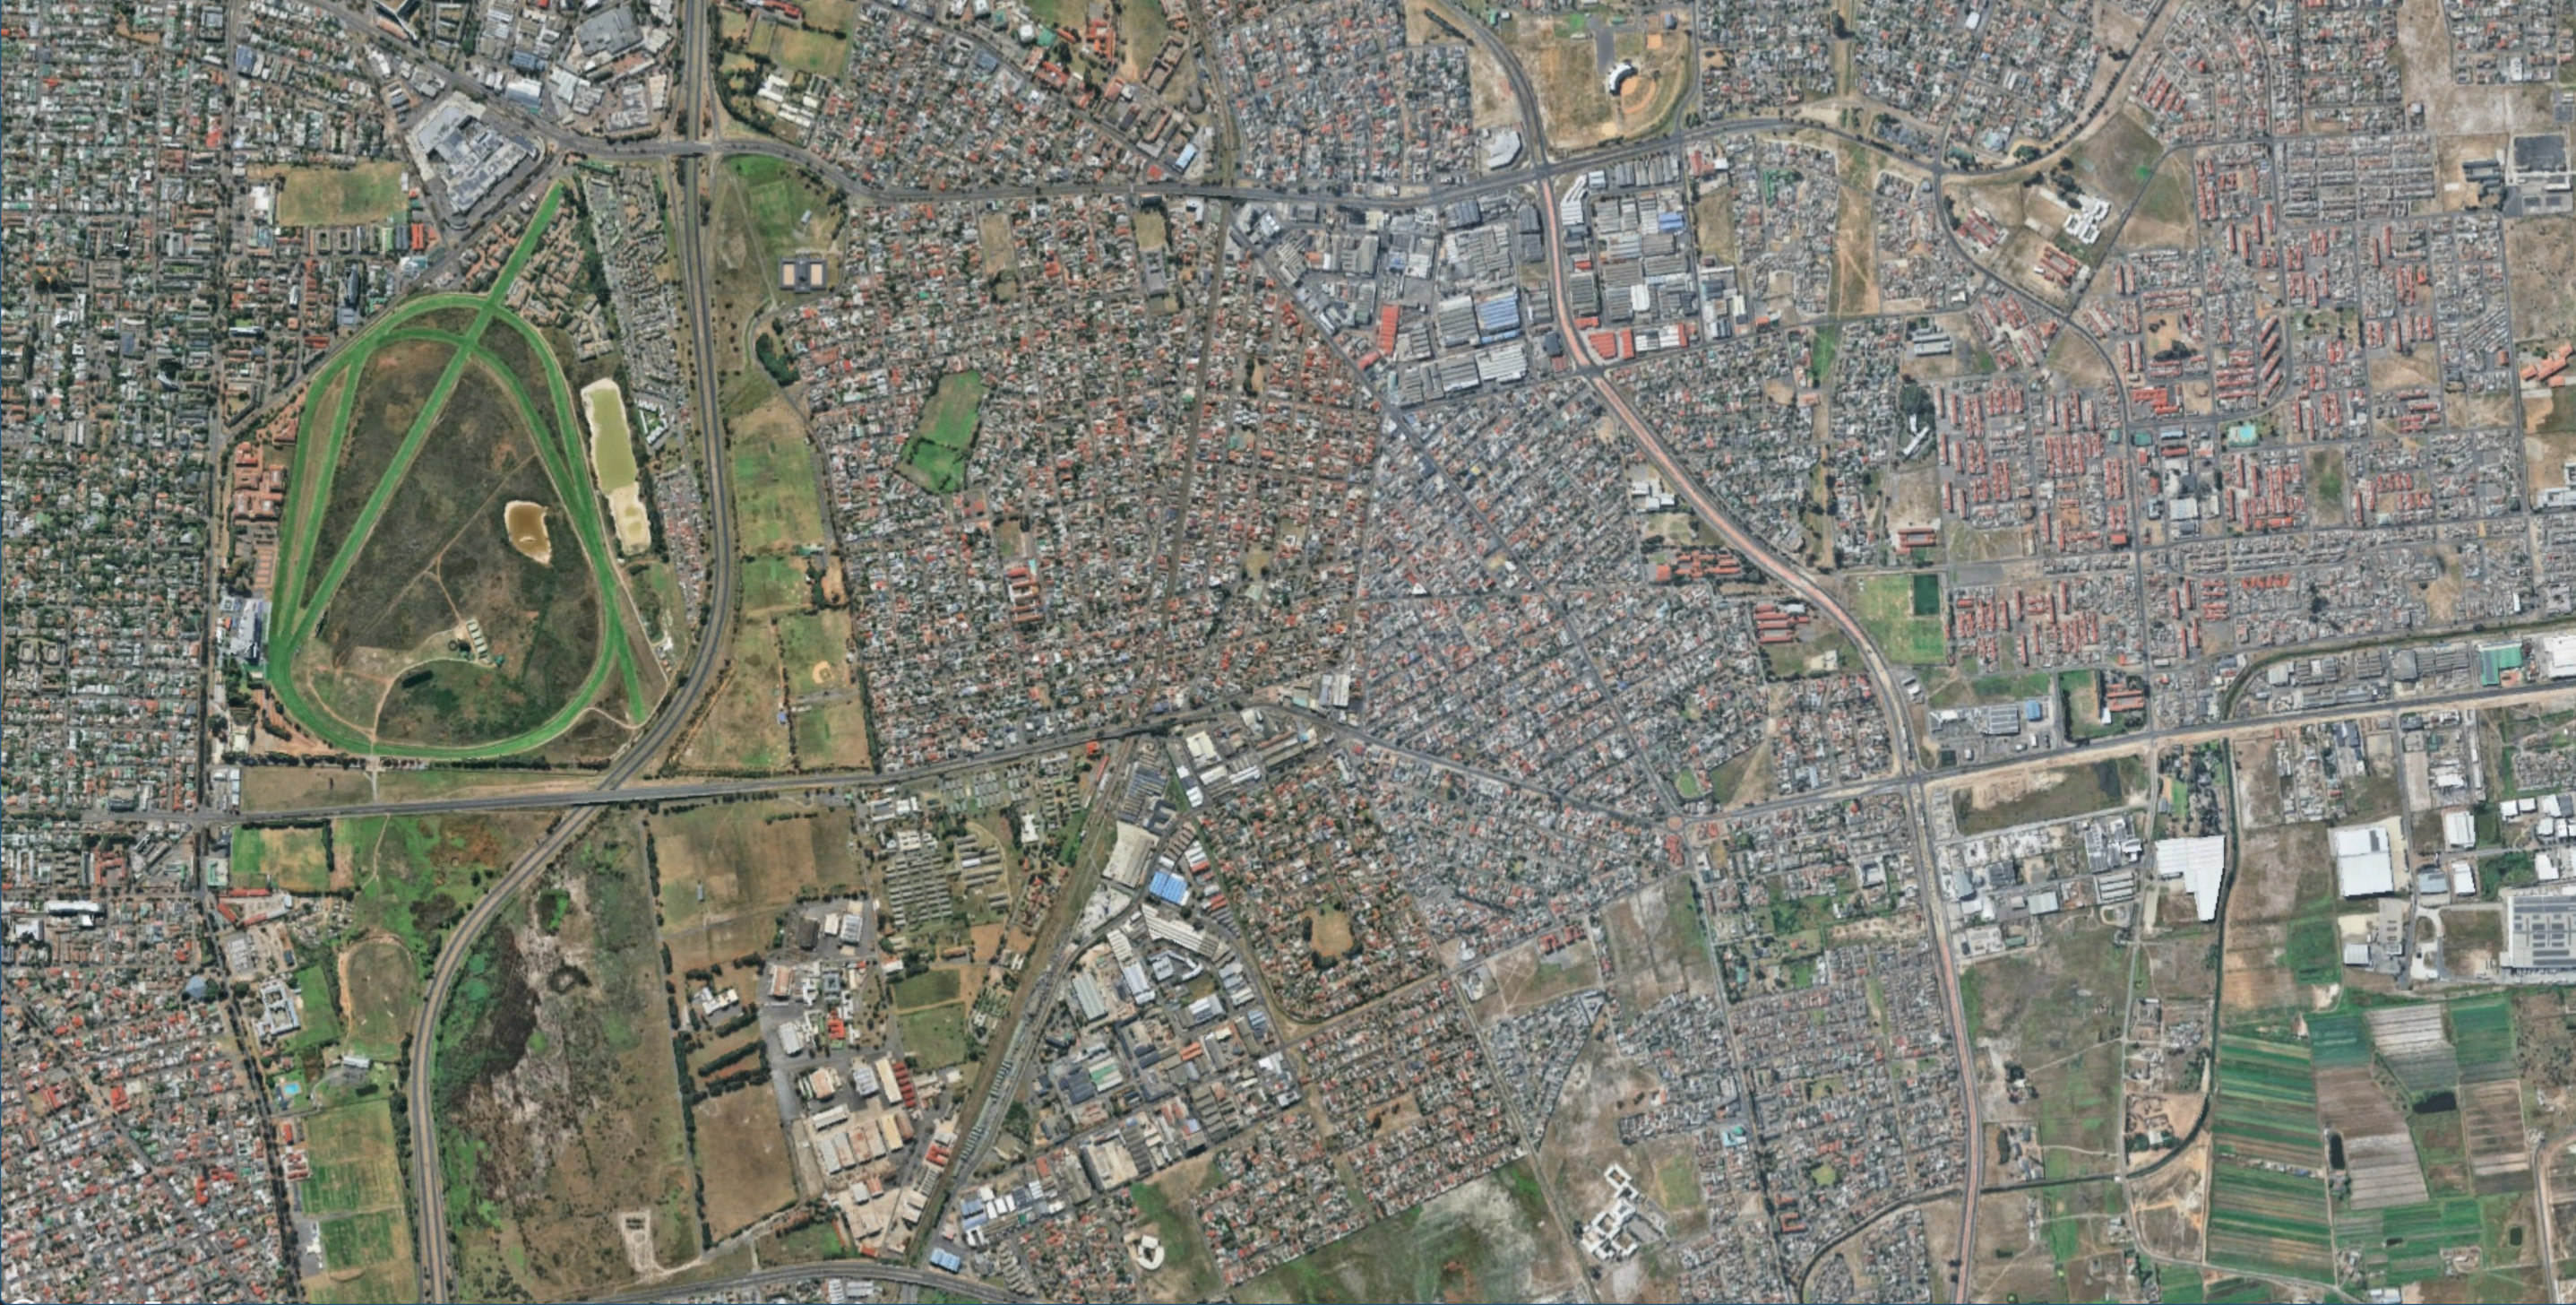
\includegraphics[width=\textwidth]{Chapter 5/RESULTPLOTS/lighting/CPTdayeg.png}
        \caption{Daytime Image of Cape Town}
        \label{fig:Day_CPT}
    \end{minipage}\hfill
    \begin{minipage}{0.24\textwidth} % Adjust width as necessary
        \centering
        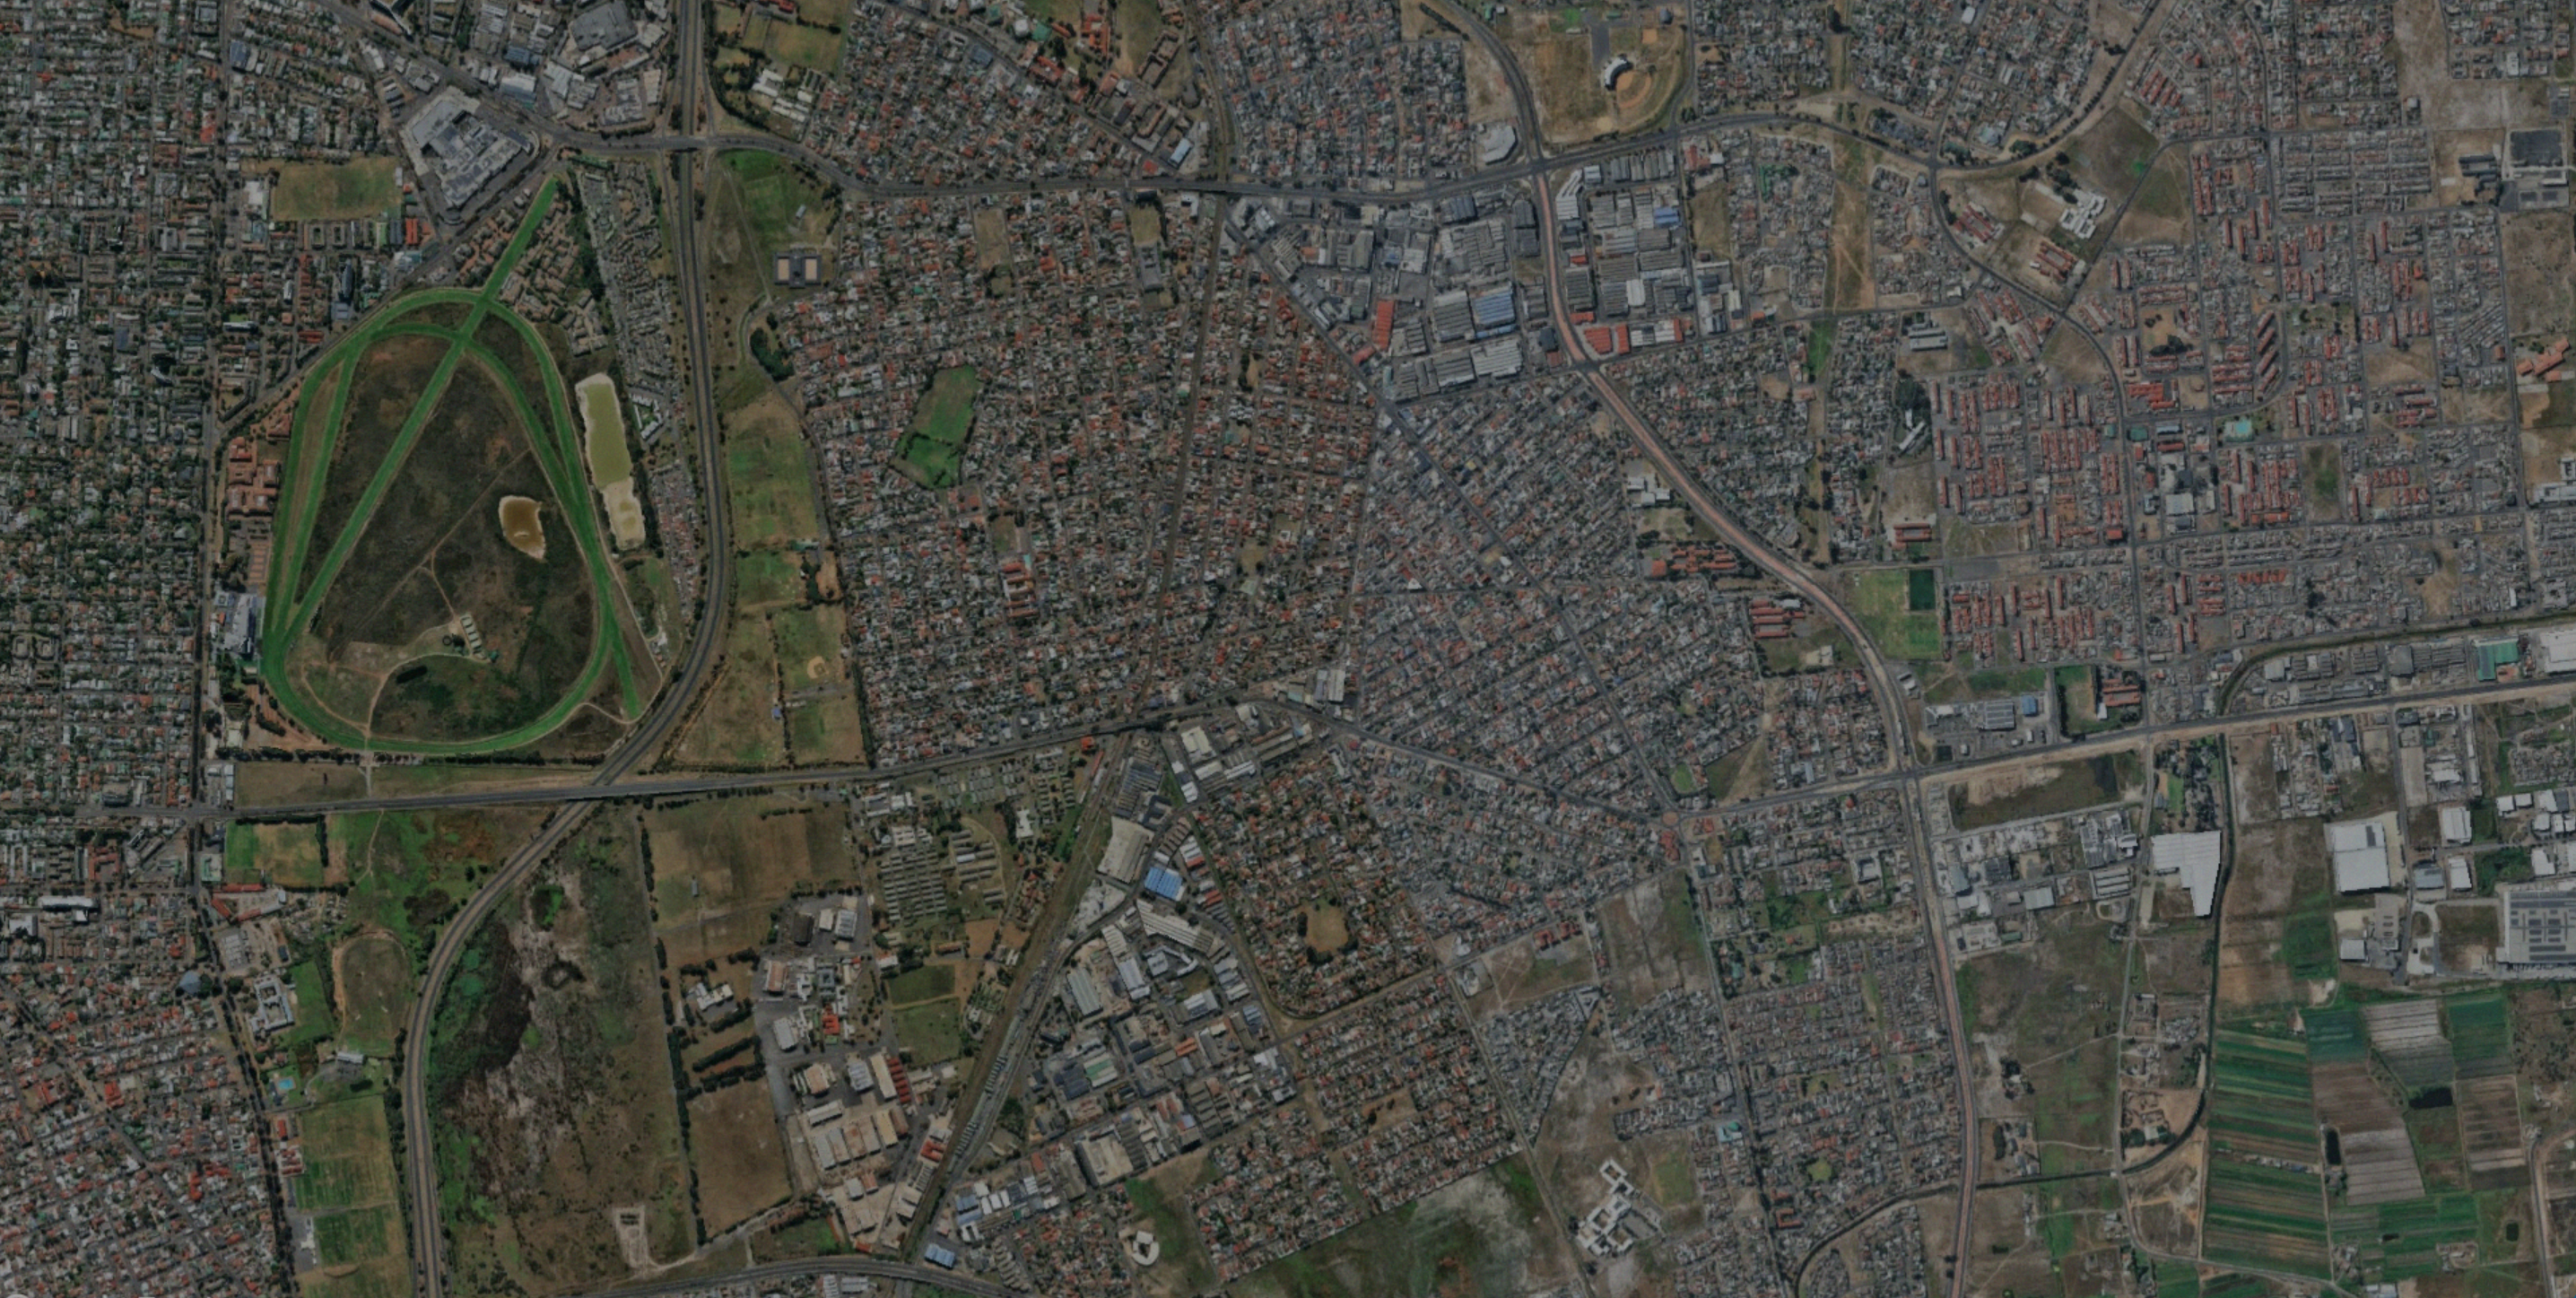
\includegraphics[width=\textwidth]{Chapter 5/RESULTPLOTS/lighting/CPTearlyeveningeg.png}
        \caption{Early Evening Image of Cape Town}
        \label{fig:Early_Evening_CPT}
    \end{minipage}\hfill
    \begin{minipage}{0.24\textwidth} % Adjust width as necessary
        \centering
        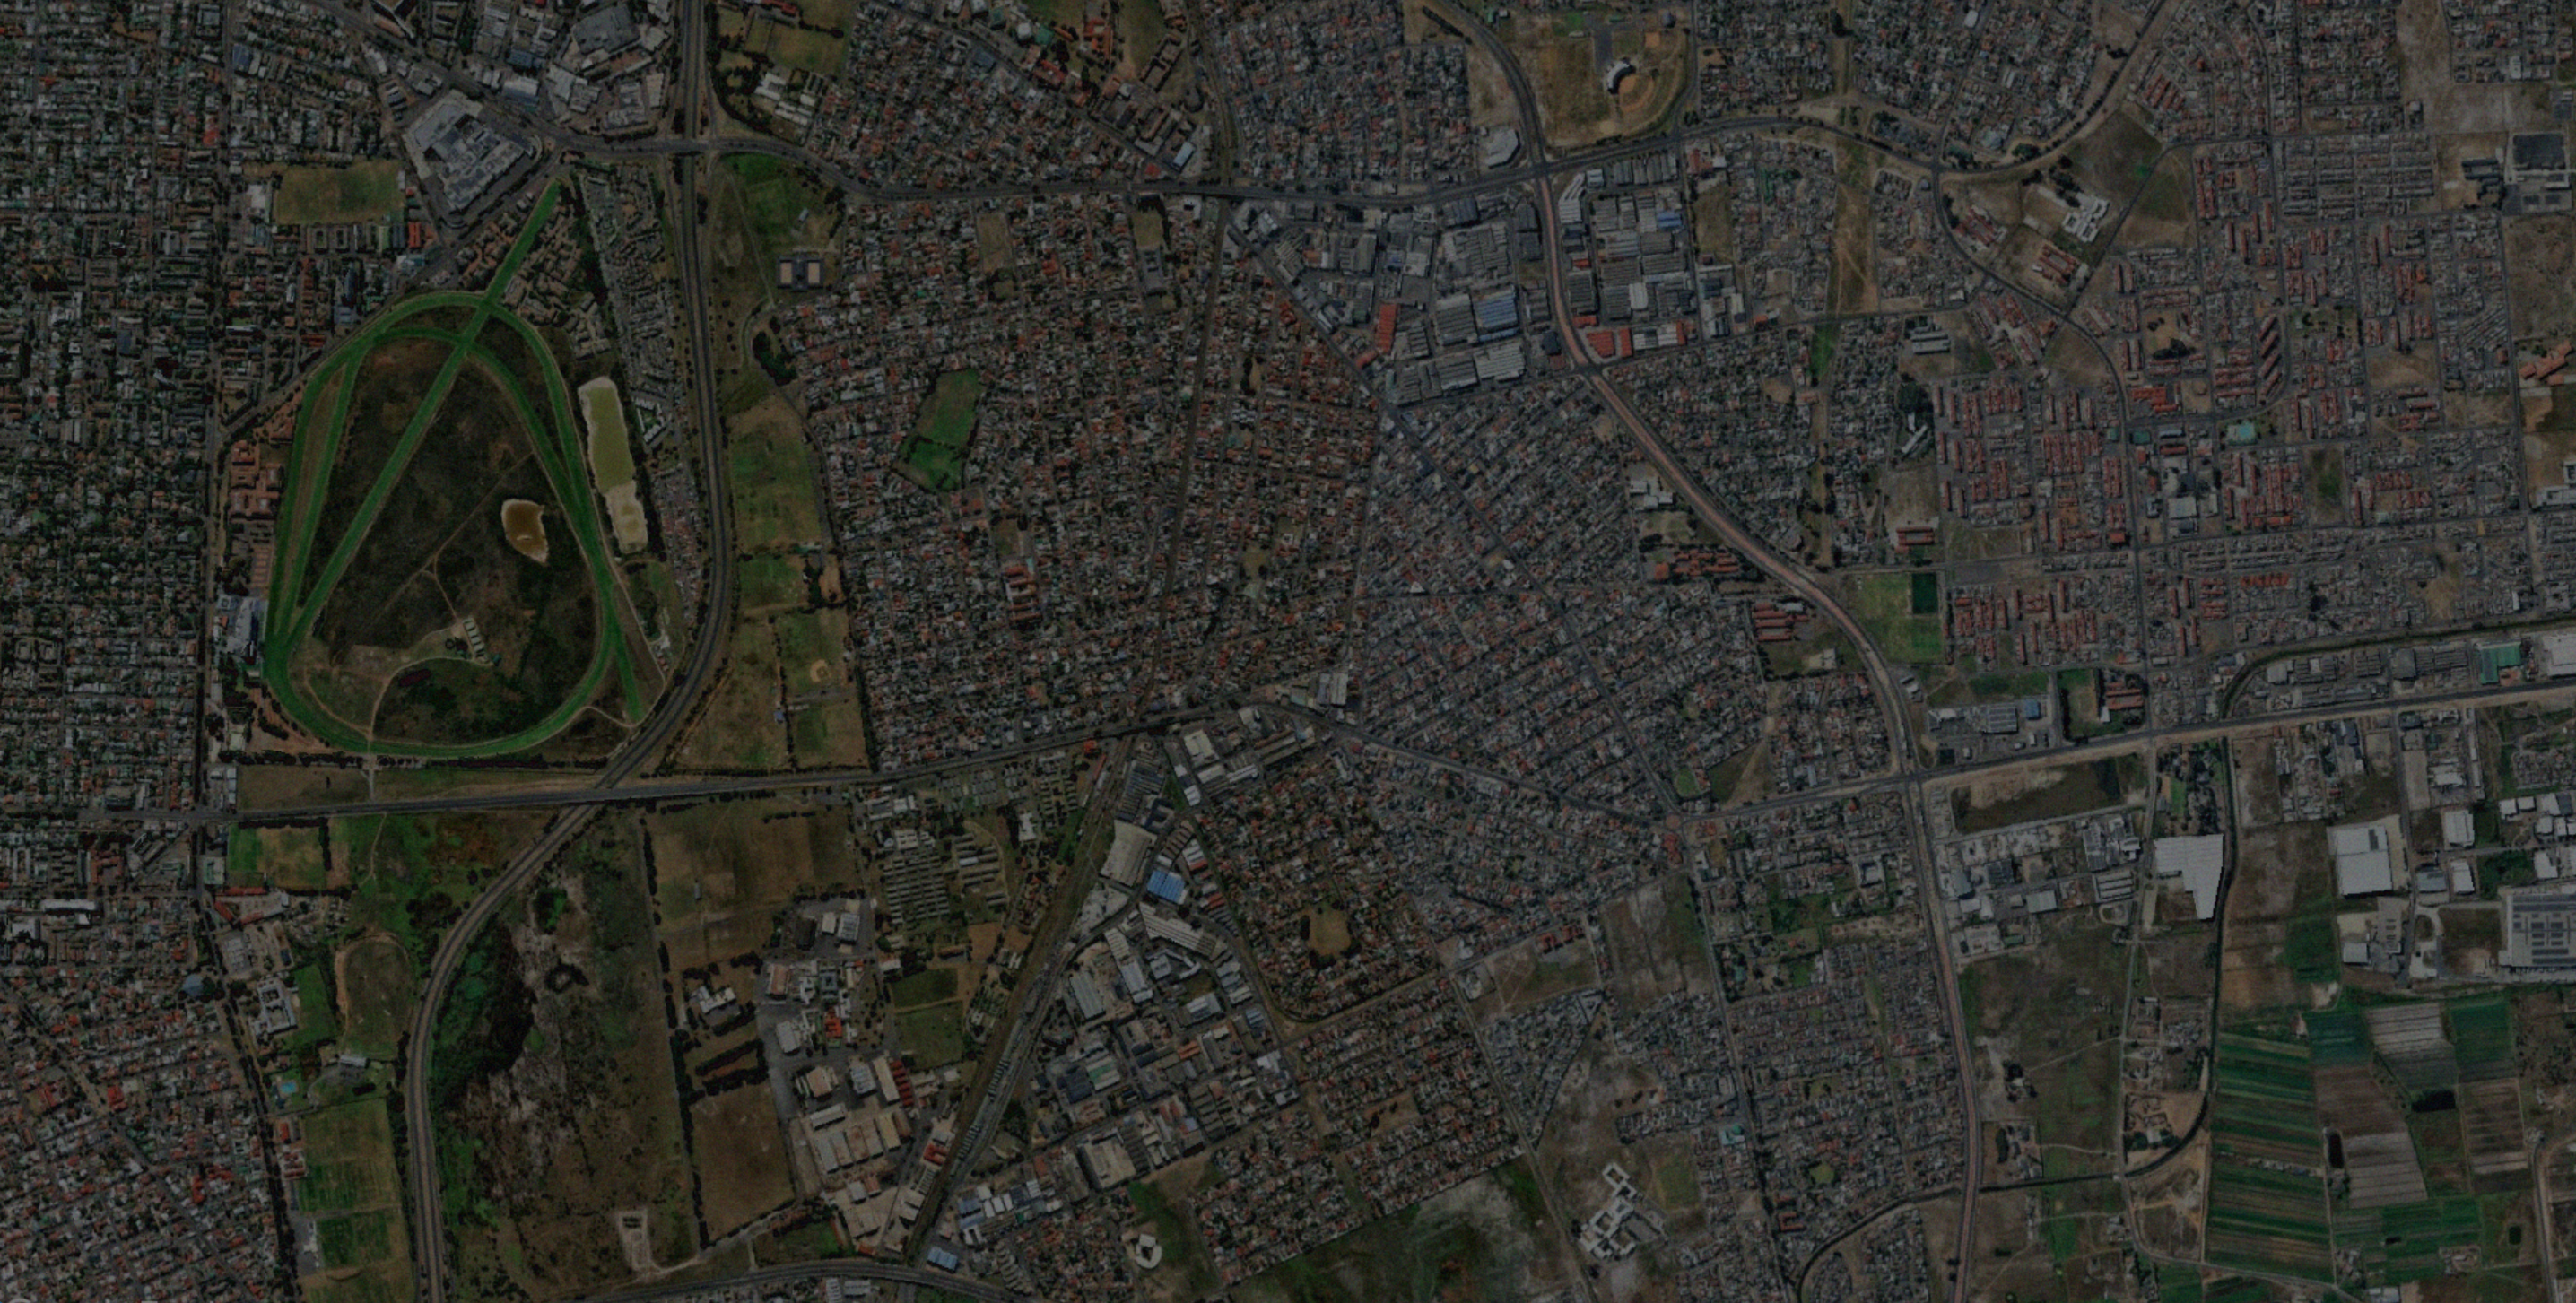
\includegraphics[width=\textwidth]{Chapter 5/RESULTPLOTS/lighting/CPTlateeveningeg.png}
        \caption{Late Evening Image of Cape Town}
        \label{fig:Late_Evening_CPT}
    \end{minipage}\hfill
    \begin{minipage}{0.24\textwidth} % Adjust width as necessary
        \centering
        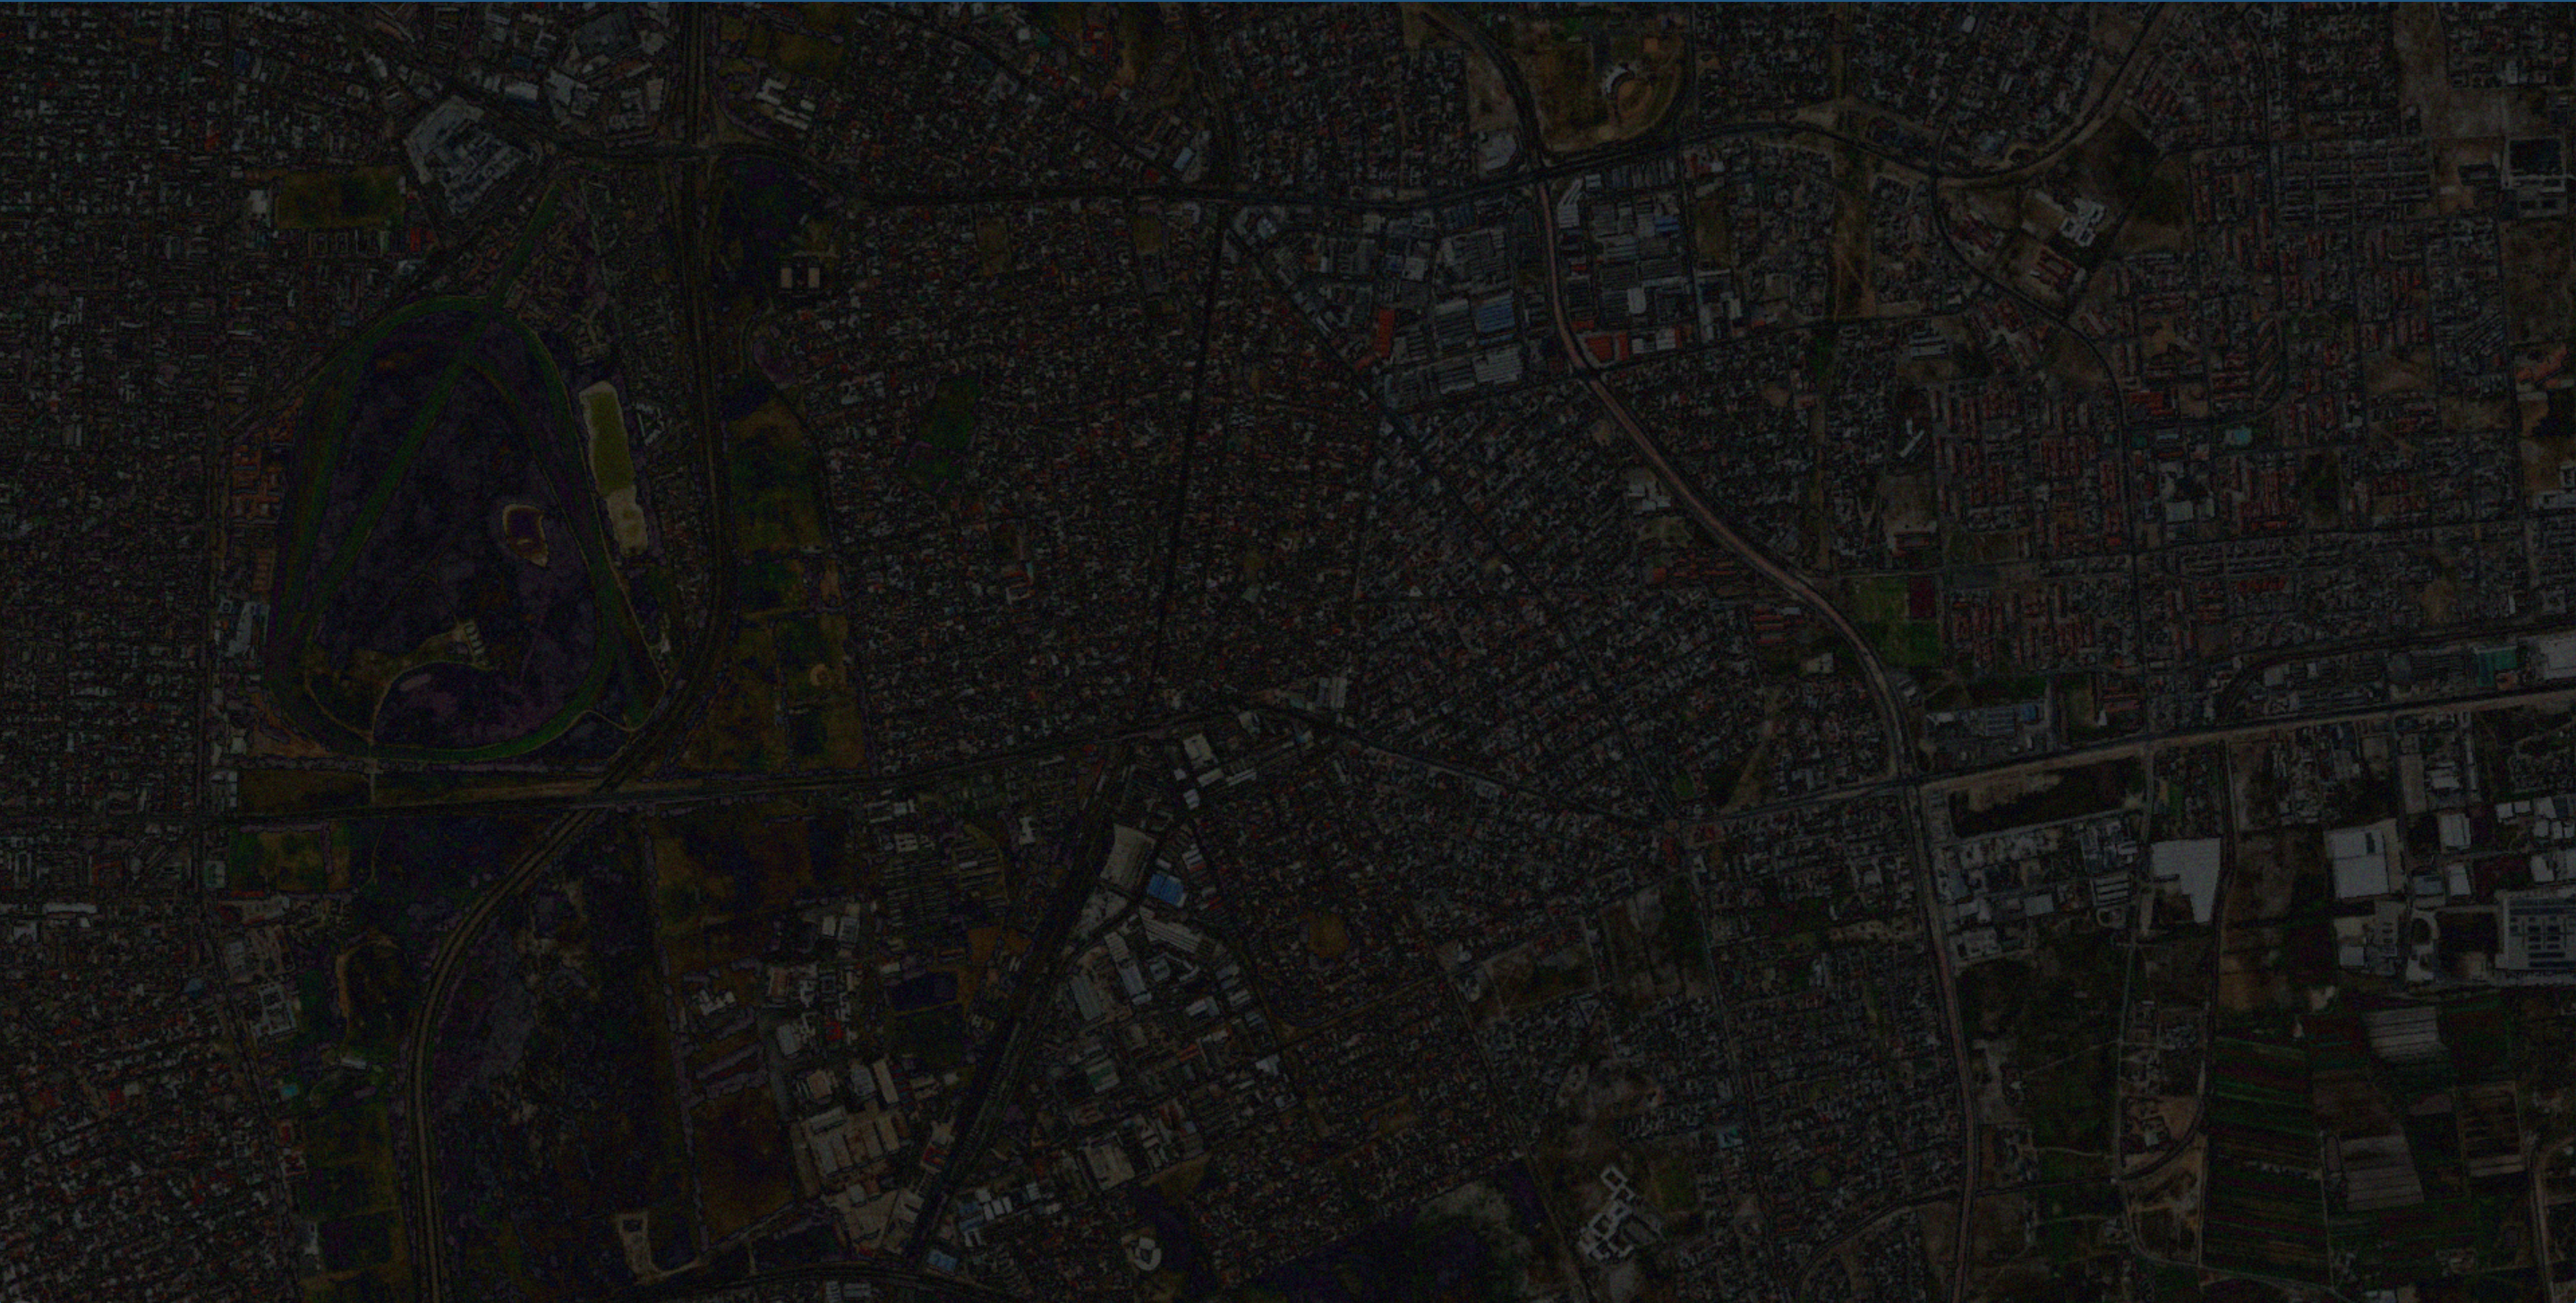
\includegraphics[width=\textwidth]{Chapter 5/RESULTPLOTS/lighting/CPTnighteg.png}
        \caption{Night Image of Cape Town}
        \label{fig:Night_CPT}
    \end{minipage}
    
    \caption{Lighting Conditions in Cape Town}
    \label{fig:Lighting_CPT}
\end{figure}


\subsubsection{Results}


Here's a polished version of the paragraph:

Figure \ref{fig:night_evening_rmse} illustrates the percentage increase in error, compared to daytime conditions, of the navigation method under early evening, late evening, and nighttime settings for each dataset.

The CITY1 dataset shows the smallest increase in error across all conditions, maintaining an error increase under 10\%. CITY2 follows with slightly higher increases in error as lighting conditions become more challenging. This could be attributed to the dataset's minimal rotations, which do not implicitly remove non-mutual information and thereby reduce false positives under difficult conditions, as is the case with the CITY1 dataset. The strong performance of the CITY datasets can be attributed to their dense feature environments with numerous high-contrast elements. However, in real-world scenarios, city lights—unaccounted for due to dataset limitations—could introduce dynamic changes impacting accuracy, especially if they occupy a significant portion of the view.

The ROCKY dataset ranks third in performance, with the DESERT and AMAZON datasets experiencing the largest increases in error. The substantial error rise in these datasets is due to their already sparse environments becoming even more feature-poor under low-light conditions, significantly increasing navigation error. The midnight and late evening settings are particularly challenging, with errors exceeding 100 times the baseline daytime error in these sparse environments.

Despite the high relative error percentages, baseline errors are typically below 1\% for most datasets, with only ROCKY exceeding 2\%. This means that, under early evening conditions, the relative error remains below 5\% for all datasets. In denser environments like the CITY datasets, errors remain under 2\% across all lighting conditions. For sparser environments, it is important to mitigate illumination changes during image capture, although the pipeline demonstrates robustness to these variations.


\begin{figure}[H]
    \centering
    \includegraphics[width=0.7\textwidth]{Chapter 5/RESULTPLOTS/lighting/lightresults.png}
    \caption{Mean Radian Increase in Error Under Nighttime and Evening Conditions.}
    \label{fig:night_evening_rmse}    
\end{figure}


% Table for Mean Radial Percentages for Different Lighting Conditions
\begin{table}[H]
    \centering
    \begin{tabular}{|c|c|c|c|c|}
    \hline
    \textbf{Dataset} & \textbf{Day (\%)} & \textbf{Early Eve (\%)} & \textbf{Late Eve (\%)} & \textbf{Midnight (\%)} \\
    \hline
    CITY1 & 0.362 & 0.363 & 0.365 & 0.371 \\
    CITY2 & 0.219 & 0.222 & 0.225 & 0.310 \\
    ROCKY & 1.909 & 2.071 & 2.290 & 20.399 \\
    DESERT & 0.251 & 0.425 & 28.713 & 112.610 \\
    AMAZON & 0.381 & 0.578 & 141.647 & 153.678 \\
    \hline
    \end{tabular}
    \caption{Mean Radial Percentages for Different Datasets under Varying Lighting Conditions}
    \label{tab:mean_radial_percent}
    \end{table}
    



    

\section{Results Conclusion}

The results presented in this chapter confirm that the system meets the accuracy and time requirements established in the objectives. The system demonstrated consistent and strong accuracy and runtime performance across various datasets, including sparse-feature environments, showcasing its ability to generalize effectively. Despite large variations in the terrains as well as other practical limitations faced, the pipeline demonstrated remarkable resilience. Further, in reality, once the path is found, there will be significantly less translation between the current and reference images, leading to a lower error ceteris paribus.


Further, the applied stress tests showed the pipelines invariance to 

The analysis further indicates that accuracy would be significantly improved with access to accurate ground truth headings and known camera parameters, reducing potential sources of error. Furthermore, the system showed resilience under challenging conditions, including low-light scenarios and images with reduced mutual information. Even with limited pixel overlap, the system continued to deliver reliable navigation data.

Overall, the system has proven to be a versatile and effective solution for UAV navigation, capable of sustaining performance under a wide range of operational challenges and environmental conditions.

